%%%%%%%%%%%%%%%%%%%%%%%%%%%%%%%%%%%%%%%%%
% Journal Article
% LaTeX Template
% Version 1.4 (15/5/16)
%
% This template has been downloaded from:
% http://www.LaTeXTemplates.com
%
% Original author:
% Frits Wenneker (http://www.howtotex.com) with extensive modifications by
% Vel (vel@LaTeXTemplates.com)
%
% License:
% CC BY-NC-SA 3.0 (http://creativecommons.org/licenses/by-nc-sa/3.0/)
%
%%%%%%%%%%%%%%%%%%%%%%%%%%%%%%%%%%%%%%%%%

%----------------------------------------------------------------------------------------
%	PACKAGES AND OTHER DOCUMENT CONFIGURATIONS
%----------------------------------------------------------------------------------------

\documentclass[twoside,twocolumn]{article}

\usepackage{blindtext} % Package to generate dummy text throughout this template 

\usepackage[sc]{mathpazo} % Use the Palatino font
\usepackage[T1]{fontenc} % Use 8-bit encoding that has 256 glyphs
\linespread{1.05} % Line spacing - Palatino needs more space between lines
\usepackage{microtype} % Slightly tweak font spacing for aesthetics

\usepackage[english]{babel} % Language hyphenation and typographical rules

\usepackage[hmarginratio=1:1,top=32mm,columnsep=20pt]{geometry} % Document margins
\usepackage[hang, small,labelfont=bf,up,textfont=it,up]{caption} % Custom captions under/above floats in tables or figures
\usepackage{booktabs} % Horizontal rules in tables

\usepackage{lettrine} % The lettrine is the first enlarged letter at the beginning of the text

\usepackage{enumitem} % Customized lists
\setlist[itemize]{noitemsep} % Make itemize lists more compact

\usepackage{abstract} % Allows abstract customization
\renewcommand{\abstractnamefont}{\normalfont\bfseries} % Set the "Abstract" text to bold
\renewcommand{\abstracttextfont}{\normalfont\small\itshape} % Set the abstract itself to small italic text

\usepackage{titlesec} % Allows customization of titles
\renewcommand\thesection{\Roman{section}} % Roman numerals for the sections
\renewcommand\thesubsection{\roman{subsection}} % roman numerals for subsections
\titleformat{\section}[block]{\large\scshape\centering}{\thesection.}{1em}{} % Change the look of the section titles
\titleformat{\subsection}[block]{\large}{\thesubsection.}{1em}{} % Change the look of the section titles

\usepackage{fancyhdr} % Headers and footers
\pagestyle{fancy} % All pages have headers and footers
\fancyhead{} % Blank out the default header
\fancyfoot{} % Blank out the default footer
\fancyhead[C]{Running title $\bullet$ May 2016 $\bullet$ Vol. XXI, No. 1} % Custom header text
\fancyfoot[RO,LE]{\thepage} % Custom footer text

\usepackage{titling} % Customizing the title section

\usepackage{hyperref} % For hyperlinks in the PDF
\usepackage[utf8]{inputenc}
\usepackage[pdftex]{graphicx}
\usepackage{minted}

\usepackage{glossaries}

%----------------------------------------------------------------------------------------
%	TITLE SECTION
%----------------------------------------------------------------------------------------

\setlength{\droptitle}{-4\baselineskip} % Move the title up

\pretitle{\begin{center}\Huge\bfseries} % Article title formatting
\posttitle{\end{center}} % Article title closing formatting
\title{Comando, control y telemetría satelital sobre lenguajes de propósito general} % Article title
\author{%
\textsc{Pablo Soligo}\thanks{A thank you or further information} \\[1ex] % Your name
%\normalsize Universidad Nacional de La Matanza - Comisión Nacional de Actividades Espaciales \\ % Your institution
%\normalsize \href{mailto:psoligo@unlam.edu.ar}{psoligo@unlam.edu.ar} % Your email address
%\and % Uncomment if 2 authors are required, duplicate these 4 lines if more
%\textsc{Jane Smith}\thanks{Corresponding author} \\[1ex] % Second author's name
%\normalsize University of Utah \\ % Second author's institution
%\normalsize \href{mailto:jane@smith.com}{jane@smith.com} % Second author's email address
}
\date{\today} % Leave empty to omit a date
\renewcommand{\maketitlehookd}{%
\begin{abstract}
\noindent 
%\blindtext % Dummy abstract text - replace \blindtext with your abstract text
Este trabajo presenta los resultados de las experiencias obtenidas en el desarrollo de un segmento terreno de próxima generación.  Se desarrolló como parte de la materia proyecto integrador de la Maestría en Desarrollos Informáticos de Aplicación Espacial (MDIAE). Teniendo como objetivo el comando y control del satélite (SCC) y la recepción de telemetría, se aplicaron técnicas y herramientas como camino alternativo al desarrollo sobre lenguajes específicos. Utilizando Python como lenguaje y aprovechado sus capacidades de reflexión, se desarrolló un entorno multimisión capaz de interpretar secuencias de comandos, incluyendo todas las estructuras de control y disponibilizando todas las capacidades del interprete. Utilizando Django como Framework y específicamente su Object Relation Mapping (ORM) se logra generar scripts de comandos con acceso simplificado a los diccionarios de comandos y valores de telemetría mediante un lenguaje estándar, de propósito general, multiplataforma y con una importante base de usuarios. Como segmento de vuelo se a utilizado satélite de formación 2017 (FS2017) que también forma parte del proyecto integrador en conjunto con las Maestría en Tecnología Satelital (MTS) y la Maestría en Instrumentos Satelitales (MIS). 
\end{abstract}
}

%----------------------------------------------------------------------------------------

\begin{document}

% Print the title
\maketitle

%----------------------------------------------------------------------------------------
%	ARTICLE CONTENTS
%----------------------------------------------------------------------------------------

\section{Introducción}

En la industria cuando se trata de comandar un equipo remoto existen varios enfoques dependiendo de las necesidades. Desde sencillas implementaciones \textit{Maestro-Esclavo} sin ningún tipo lógica asociada, pasando por sistemas algo mas complejos donde se aplican restricciones o sistemas basados en maquinas de estado. En el área espacial, una práctica común es el uso de secuencias de comandos sobre estructuras de control. Empresas y agencias espaciales en todo el mundo han desarrollados sus propios lenguajes e intérpretes para cumplir con este objetivo: 

\begin{description}
 \item [STOL:] Satellite Test and Operation Language. Desarrollado por la Nasa y ampliamente utilizado en varias misiones. 
 \item [PLUTO:] presente en algunas misiones de la ESA (Satellite Control and Operation System 2000).
 \item [Otros:] desarrollados o utilizados por diferentes compañias  SOL(GMV), CCL(Harris), PIL(Astrium), SCL(ICS). 
\end{description}

En el caso del segmento terreno del FS2017 se optó por usar un lenguaje de propósito general en lugar de crear un lenguaje especifico
o utilizar los existentes en CONAE (Comisión Nacional de Actividades Espaciales). Este enfoque presenta múltiples ventajas,

\begin{description}
 \item [Portabilidad: ] escogiendo correctamente la herramienta se puede lograr una buena portabilidad entre distintas plataformas.
 \item [Capacidad: ] las herramientas y capacidades generales de un buen lenguaje y entorno de desarrollo de propósito general superan ampliamente las posibilidades que puede ofrecer un entorno de propósito especifico.
 \item [Base de usuarios: ] una importante base de usuarios implica soporte, documentación y mejoras ademas de una base de posibles recursos ya capacitados. 
\end{description}

En el caso del proyecto integrador la opción de lenguaje propio de la misión se descartó por no disponer del tiempo que implica desarrollar y validar un intérprete de propósito específico. La opción de utilizar los interpretes de CONAE quedó relegada por sobre la opción Python, con una base de usuarios mucho más grande, multiplataforma, con capacidades de depuración, documentación y de dominio de todos los estudiantes. 


%------------------------------------------------


%------------------------------------------------
\section{Arquitectura}
La solución propuesta se basa en una arquitectura cliente-servidor estándar y esta influenciada por el framework de desarrollo Django, el que también influyo en un análisis y diseño orientado a objetos. Como repositorio de datos se utiliza un Postgresql 9.0 donde se almacenan la definición de datos y los datos mismos. Todo el acceso se realiza mediante el ORM y no hay en todo el software un acceso directo al motor. Los componentes de software son los siguientes:

\begin{description}
 \item [Database server (1): ] Un servidor SQL Postgres donde se almacenan la definición de telemetría, telecomandos y los datos para todas las misiones.  
 \item [Application server (1): ] Un servidor de aplicación responsable de la generación de interfaces y lógica de operación.
 \item [Telemetry and Telecomand Processor (n): ] modulo encargado de decodificar, calibrar y transformar en variables de ingeniería la telemetría según su definición y de codificar y enviar los comandos al segmento de vuelo. En este caso existe un proceso por satélite incluso si son del mismo fabricante. Para el caso de \textit{FS2017} debe conectar al puerto 3210 por TCP/IP tanto para recibir telemetría como para el envío de comandos.
\end{description}

La figura \ref{fig:Arq01} muestra un esquema de alto nivel de la arquitectura.

\begin{figure}[]
  \caption{Arquitectura}
  \label{fig:Arq01}
  \centering
  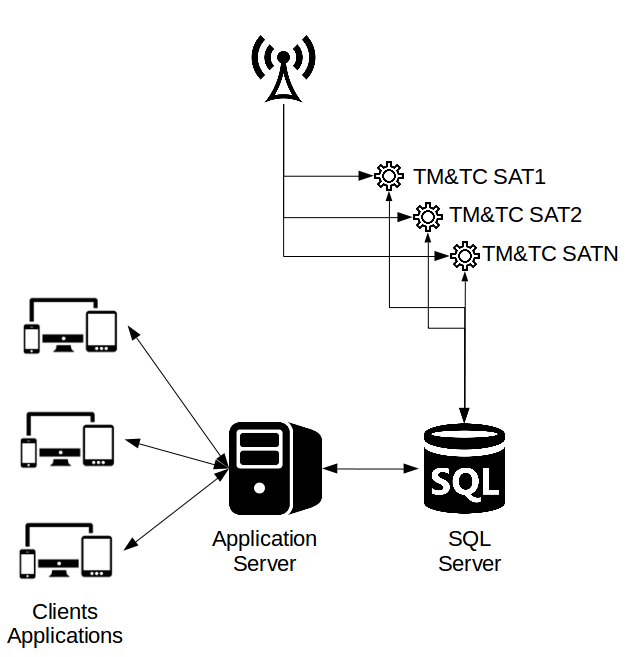
\includegraphics[width=0.4\textwidth]{Imagenes/Arq01.png}
\end{figure}



\section{Python y Django}

Python es un lenguaje portable, abierto, de alto nivel es dinámico y tiene orientación a objetos no estricta. (Permite programación estructurada). Concebido durante los 80 se popularizó en los 90, muestra una performance superior a otros interpretes, producto de su código intermedio (bytecode). Además de la portabilidad, que no mostró ninguna fisura, su punto fuerte es la gran comunidad que brinda soporte y la buena integración con entornos de desarrollo como Eclipse.  El lenguaje tiene buena productividad \cite{prechelt2000empirical}, estructuras complejas de datos ya incorporadas, manejo de excepciones, recolector de basura y capacidad de reflexión, mandatoria para cumplir con el objetivo. Otros beneficios de trabajar con Python, o con otro lenguaje maduro de propósito general, son las capacidades de depuración, los test unitarios y la generación de documentación automatizada. Este enfoque además permite pleno acceso a herramientas de comunicación como Sockets, http, RPC (Remote Procedure Call), Web Services, email y a bibliotecas de manejo de archivos XML entre otros. 
Django es el framework web para python más popular, además de ofrecer herramientas para el desarrollo web incorpora un robusto ORM que se ha usado intensivamente en todos los módulos del segmento terreno, incluyendo los que no tienen interfaces web. Django propone un desarrollo basado en modelos, con una orientación a objetos estricta, pudiendo aprovechar las capacidades de abstracción, herencia, polimorfismo y las ventajas de un mejor modelo de reusabilidad. El acceso al motor de base de datos es transparente al desarrollador de la aplicación como al operador que realiza los scripts de comandos, toda la responsabilidad sobre la recuperación y persistencia de datos recae sobre el ORM.  


\section{Telemetría}
\label{sec:telemetria}

Para el caso del FS2017 la telemetría se recibe en tramas AX.25 por TCP/IP \footnote{Alternativamente se puede obtener por puerto serie} puerto 3210 según especificación del fabricante. La trama tiene un fragmento de \textit{Payload} donde viene codificada la telemetría. La definición de la telemetría esta persistida en la entidad \textit{TlmyVarType} donde se establece el tipo, valor, rangos, límites, posición dentro de la trama y la función que la transforma en una variable de ingeniería. En el área satélite y en algunos sistemas de control y automatización es común recibir la telemetría en valores crudos o \textit{raw}. A estos valores crudos se les debe aplicar una función que los transforme en unidades de ingeniería. En algunas áreas, incluida la satelital,  esta transformación también es utilizada para calibrar sensores o equipos que puedan sufrir desgaste o variaciones por las condiciones de uso. Estos ajustes pueden ir desde un simple ajuste por función lineal hasta una discretización de valores por tablas de \textit{look-up}. El sistema debe ser lo suficientemente flexible como para permitir aplicar cualquier función de transformación a toda variable de telemetría y permitir ajustarla a medida que el desgaste de los sensores lo requiera.
La figura \ref{fig:MetodoCalibracion} muestra como al configurar una variable de telemetría se selecciona la función a aplicar para convertirla en variable de ingeniería.

\begin{figure}[]
  \caption{Selección de método de calibración}
  \label{fig:MetodoCalibracion}
  \centering
  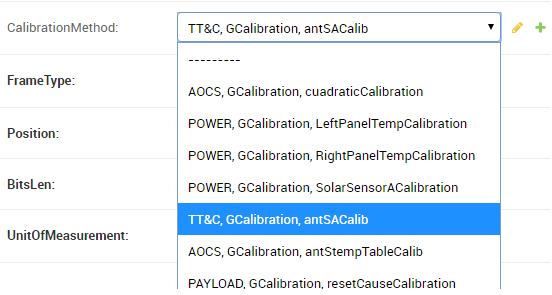
\includegraphics[width=0.5\textwidth]{Imagenes/TTCCalibracionDiscreta.png}
\end{figure}

Mediante técnicas de reflexión se carga en tiempo de ejecución la función seleccionada de calibración y se le aplica al valor \textit{raw} extraído de la trama de telemetría proveniente del paquete AX.25. La función de calibración puede ser cualquier secuencia de comandos programable en python sin ningún tipo de restricción mas allá del tiempo de procesamiento. Todas las bibliotecas y estructuras de datos están disponibles incluyendo funciones matemáticas e incluso el acceso al la base de datos completa mediante ORM.
Al tener acceso a la base de datos se pueden obtener coeficientes actualizados de calibración permitiendo: 

\begin{description}
 \item [Reutilizar funciones: ] es posible crear una única función para ajustes típicos (lineal, cuadrático) y reutilizarla con distintos coeficientes según la variable de telemetría requiera.
 \item [Calibración fina: ] creada una función modificando los coeficientes se puede realizar un ajuste fino, por ejemplo por desgaste de un sensor, sin necesidad de recodificar la misma.
\end{description}

Como ejemplo el segmento de vuelo \textit{FS2017} requiere que a muchos de sus valores crudos se les aplique una ganancia +/- un desplazamiento u \textit{offset}. En todos los casos se realiza mediante una única función llamada \textit{linealCalibration} aunque cada tipo de variable de telemetría posea sus propios valores para ambos coeficientes.

Para que un método sea considerado de calibración o ajuste debe estar desarrollado como método de una clase heredada de \textit{BaseCalibration}. El software realiza una exploración de todos los métodos públicos de clases derivadas de \textit{BaseCalibration} y los disponibiliza para su aplicación a las distintas variables de telemetría \ref{fig:MetodoCalibracion}. La figura \ref{fig:GCalibration} muestra la clase \textit{GCalibration}, heredada de \textit{BaseCalibration}, donde se implementan algunos métodos de calibración incluido el seleccionado en la figura \ref{fig:MetodoCalibracion}.

\begin{figure}[!htb]
    \centering
    \begin{minipage}{0.2\textwidth}
        \centering
        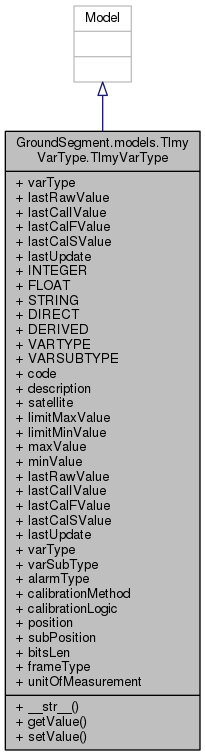
\includegraphics[width=0.5\linewidth]{Imagenes/TelemetryVarType.png}
        \caption{Clase TlmyVarType}
        \label{fig:prob1_6_2}
    \end{minipage}%
    \begin{minipage}{0.2\textwidth}
        \centering
        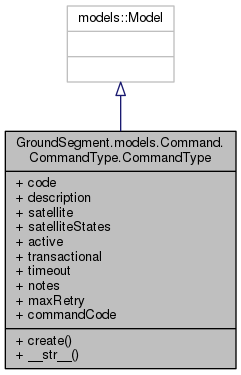
\includegraphics[width=0.5\linewidth]{Imagenes/CommandType.png}
        \caption{Clase CommandType}
        \label{fig:prob1_6_1}
    \end{minipage}
\end{figure}

El siguiente código muestra parte de la implementación del método \textit{setValue} de la clase \textit{TlmyVar}. 


\begin{minted}[fontsize=\tiny]{python}
class TlmyVar(models.Model):
  ...
  if raw!=self.tmlyVarType.lastRawValue:
    self.tmlyVarType.lastRawValue = raw
    if self.tmlyVarType.calibrationMethod: 
      if not self.tmlyVarType.calibrationLogic:
	  klass = 
	    globals()[self.tmlyVarType.calibrationMethod.aClass]
	  instance = klass()
	  methodToCall = 
	    getattr(instance, 
		    self.tmlyVarType.calibrationMethod.aMethod)
	    self.tmlyVarType.calibrationLogic = 
	      methodToCall
      else:
	  pass #Calibracion ya cargada   
      
      if self.tmlyVarType.varType==self.tmlyVarType.INTEGER:
	  self.tmlyVarType.lastCalIValue = 
	    self.tmlyVarType.calibrationLogic(self.tmlyVarType,  raw )

      elif self.tmlyVarType.varType==self.tmlyVarType.FLOAT:
	  self.tmlyVarType.lastCalFValue = 
	    self.tmlyVarType.calibrationLogic(self.tmlyVarType,  raw )
      else:
	  self.tmlyVarType.lastCalSValue = 
	    self.tmlyVarType.calibrationLogic(self.tmlyVarType,  raw )
    else:
	if self.tmlyVarType.varType==self.tmlyVarType.INTEGER:
	    self.tmlyVarType.lastCalIValue = raw
	elif self.tmlyVarType.varType==self.tmlyVarType.FLOAT:
	    self.tmlyVarType.lastCalFValue = raw
	else:
	    self.tmlyVarType.lastCalSValue = raw 
	
    """			
    Si el tipo no es cadena llevo el dato a cadena
    """
    value = self.tmlyVarType.getValue()
    
    if self.tmlyVarType.varType!=self.tmlyVarType.STRING:
	if (value>=self.tmlyVarType.limitMaxValue and 
	    value<=self.tmlyVarType.limitMinValue):
	    raise Exception("Invalid value in var "+
	                     self.tmlyVarType.code)  
	
    if saveifchange:
	self.tmlyVarType.lastUpdate = datetime.now(utc)
	self.tmlyVarType.save()

    
    if self.tmlyVarType.varType==self.tmlyVarType.INTEGER:
	self.calIValue = self.tmlyVarType.lastCalIValue
	self.calSValue = str(self.calIValue)
    elif self.tmlyVarType.varType==self.tmlyVarType.FLOAT:
	self.calFValue = self.tmlyVarType.lastCalFValue
	self.calSValue = str(self.calFValue)
    else:
	self.calSValue = self.tmlyVarType.lastCalSValue
      


    return self.tmlyVarType.getValue()

\end{minted}




Cuando se recibe un nuevo valor de telemetría se persiste mediante una instancia de \textit{TlmyVar}. Toda recepción de nueva telemetría se persiste, haya cambiado o no su valor. También se deja el ultimo valor en la variable \textit{TlmyVarType}, esta desnormalización tiene como objetivo ganar eficiencia al consultar los valores de tiempo real, en lugar de consultar a la tabla de histórica de valores recibidos, se consulta a la tabla de tipos que tiene un tamaño acotado. Si el valor raw para una variable determinada no cambio desde la ultima actualización entonces se guarda el registro de la recepción pero no se aplican las calibraciones. Esto ultimo hace ganar eficiencia ya que no se vuelve a transformar cuando se sabe que el resultado sera el mismo, se debe tener en cuenta, sin embargo, que ante un cambio en las funciones de calibración se debe forzar mediante software a una nueva evaluación aunque el raw no haya cambiado\footnote{No implementado aún}.
Si se produce un cambio en el raw se carga dinámicamente la función de ajuste \textit{self.tmlyVarType.calibrationLogic} solo si no fue cargada anteriormente. La carga del método de calibración a una atributo del tipo de variable de telemetría se realiza una única vez durante la ejecución. Esto permite ganar eficiencia pero obliga a reiniciar los el modulo de telemetría y telecomandos ante un cambios en los métodos. La figura \ref{fig:TiempoDecodificacion} muestra los tiempos de procesamiento para un bloque de 25 paquetes donde se decodifican 18 variables.

\begin{figure}[]
  \caption{Tiempo de decodificación}
  \label{fig:TiempoDecodificacion}
  \centering
  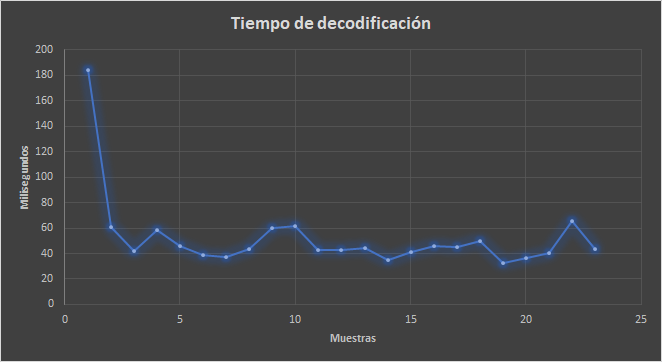
\includegraphics[width=0.5\textwidth]{Imagenes/tiempoDecodificacion.png}
\end{figure}

La primera decodificación demora mas que las siguientes dado que tiene que realizar la carga de las funciones de transformación, luego el tiempo se estabiliza alrededor de los 50 milisegundos para el conjunto de las 18 variables. El tiempo de procesamiento incluye además la verificación de que los valores de las variables de ingeniería estén dentro del rango de seguridad.




% \begin{figure}[]
%   \caption{Tipo de telemetría}
%   \label{fig:TipoTelemetria}
%   \centering
%   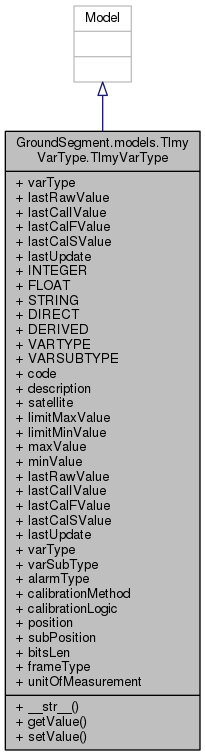
\includegraphics[width=0.2\textwidth]{Imagenes/TelemetryVarType.png}
% \end{figure}


\begin{figure}[]
  \caption{GCalibration}
  \label{fig:GCalibration}
  \centering
  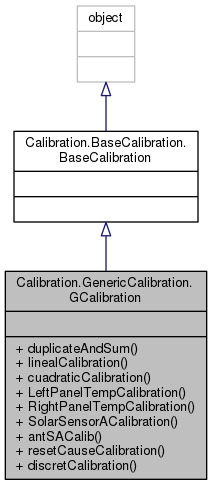
\includegraphics[width=0.2\textwidth]{Imagenes/GenericCalibration.png}
\end{figure}


El siguiente código muestra una calibración lineal (que puede ser usada en muchas tipos de variable de telemetría) y que obtiene sus coeficientes utilizando el ORM.

\begin{minted}[fontsize=\scriptsize]{python}

#Clase GCalibration hereda de BaseCalibration
class GCalibration(BaseCalibration):
    ...
  
    #Metodo generico de calibración lineal
    def linealCalibration(self, obj, raw):
	#Multiplica el valor raw por la ganancia y 
	#offset configurado para ese tipo de
	#de variable de ingeniería. Los obj tiene 
	#el tipo de variable de ingeniería y
	#por medio del ORM se accede a los 
	#valores configurados.
        return raw*
	    obj.coefficients.get(code="GAIN").value + 
	    obj.coefficients.get(code="OFFSET").value

\end{minted}

\section{Telecomandos}
\label{sec:telecomandos}

En el caso del \textit{FS2017} los telecomandos deben ser enviados al segmento de vuelo por el mismo canal en donde se recibe la telemetría, TCP/IP puerto 3210. Los comandos deben ser codificados en una trama AX.25. 
Para permitir el la creación de scripts de comandos, de la misma forma que con la telemetría \ref{sec:telemetria} se utilizaran las capacidades de reflexión para analizar en tiempo de ejecución los scripts a ejecutar. Los scripts de comandos pueden ejecutarse por acción explicita de un operador o porque fueron aplicados a una pasada. 
El operador tiene pleno acceso al ORM de donde puede obtener el diccionario de comandos y los valores de telemetría si necesitar aplicar condicionales que dependieran del estado del segmento de vuelo. Se le ha añadido al segmento terreno capacidades de operación por consola como recomienda \cite{galal2001satellite}. El siguiente código muestra como se envía un comando de encendido de \textit{heater} si la temperatura de la OBC esta por debajo de un valor determinado.

\begin{minted}[fontsize=\scriptsize]{python}

#Instancio el satélite FS2019
sat = Satellite.objects.get(code="FS2019")
...

if not sat.isConnected():
  raise Exception("Abort, flight segment offline")

#Consulto si la temperatura de la OBC esta por 
#debajo de 10 grados y tambien
#Verifico que el heater este apagado
if sat.tmlyVarType.get(code="obcT1").getValue()<10 
 and 
 sat.tmlyVarType.get(code="HeaterOn").getValue()==False:
   
   #Obtengo el tipo de comando para encender el heater
   ct = sat.getCommandType().get(code="HeaterTurnOn")
   #Creo un nuevo comando para el satelite, con fecha 
   #de vencimiento 5 minutos desde la fecha de creación. 
   #Es un comando de ejecución en tiempo real 
   #y por tanto no 
   #se agrega un tercer parametro de fecha de ejecución
   cmd = sat.newCommand(ct, 
	        datetime.utcnow()+timedelta(minutes=5))
   #Finalmente envío el comando.
   sat.sendCommand(cmd)
\end{minted}

Por consola se obtiene el satélite con el que se desea trabajar. Se consulta por la temperatura de la OBC mediante una lectura del valor en tiempo real de la variable de telemetría \textit{obcT1}. Si ese valor es inferior a 10 (El método  \textit{getValue()} siempre retorna variable de ingeniería) y los \textit{heaters} esta apagados entonces se envía un comando de encendido.
Las capacidades de las sentencias \textit{sat.tmlyVarType.get(code="obcT1")} y \textit{sat.tmlyVarType.get(code="HeaterOn")} que retornan la instancias de \textit{TlmyVarType} son provistas por el ORM de django a pesar de ser utilizadas por consola. 



\section{Resultados}
\label{sec:resultados}


\subsection{Interprete y Framework de desarrollo}
El lenguaje (python) es sencillo aprender, c

\subsection{Desarrollo multiplatafoma}
La solución fue ejecutada en ubuntu linux 15.10 como en windows 10.0 y windows 7.0. En ambos casos el software se ejecuto sin cambios. En este punto tanto el interprete como el framework mostraron uno de sus atributos mas valorables.


\subsection{ORM}
El ORM de Django se mostró estable, no se registraron problemas o \textit{bugs}. Para la creación y modificación de modelos, su flujo divido en dos etapas \footnote{Disponible en la versiones de Django iguales o superiores a 1.7} \textit{Make Migrations} y \textit{Migrate} permitió el trabajo colaborativo y con múltiples servidores. Las consultas tampoco mostraron errores pero, especialmente para el filtrado de resultados, requieren del aprendizaje de convenciones propias lo que afecta la curva de aprendizaje. No se pueden declarar atributos privados, cuestión que afecta el encapsulamiento, y la capacidad del ORM para trabajar con polimorfismo esta limitada y se requiere añadir paquetes especiales.

\subsection{Reflexión}



% \begin{table}
% \caption{Example table}
% \centering
% \begin{tabular}{llr}
% \toprule
% \multicolumn{2}{c}{Name} \\
% \cmidrule(r){1-2}
% First name & Last Name & Grade \\
% \midrule
% John & Doe & $7.5$ \\
% Richard & Miles & $2$ \\
% \bottomrule
% \end{tabular}
% \end{table}



% \begin{equation}
% \label{eq:emc}
% e = mc^2
% \end{equation}
% 


%------------------------------------------------

\section{Discusión}	

Los lenguajes específicos del sector espacial fueron creados hace décadas. Durante los 70, si bien existían opciones interpretadas , están no eran de uso extendido. En la actualidad existen varias opciones con una amplia cantidad de usuarios de base y múltiples proyectos que avalan su robustez. Python, Perl, VBScript, JavaScript son solo algunas opciones. Incluso la técnica aplicada en este trabajo es implementable, con algunas restricciones, en lenguajes compilados, siempre y cuando tengan capacidades de reflexión avanzadas. Java o C\#, herramientas que generan código intermedio son aplicables así como compilados puros. Delphi mediante su RTTI (Run-time type information) para citar un ejemplo, requeriría que los métodos de calibración sean compilados previamente para luego ser cargados dinámicamente como complementos o \textit{plug-ins} durante la ejecución del modulo principal. A esta opción se la juzga mas compleja y si bien puede ofrecer mejoras en cuanto a rendimiento, los resultados no justifican su implementación. 
Las opciones ampliamente probadas de la actualidad no justifican el desarrollo de un lenguaje propietario, no tener una base de usuarios implica ausencia de documentación, soporte, herramientas y por sobre todo recursos como explica \cite{smith2003ada} refiriéndose a ADA. ``Using Ada could potentially offer lower life cycle costs compared to other programming languages, but it seems more likely that using Ada would raise life cycle costs due to a
dearth of tools and compilers and lack of trained, experienced programmers''. La creación de una herramienta propietaria limita las capacidades disponibles en términos de estructuras de datos y bibliotecas en general y obliga a su desarrollo con el costo que esto conlleva y su aprendizaje carece de valor al ser inaplicable por fuera del ámbito donde se implemente. 


%----------------------------------------------------------------------------------------
%	REFERENCE LIST
%----------------------------------------------------------------------------------------

\newglossaryentry{raw}
{
  name=raw,
  description={Valor crudo, se le debe aplicar una función que lo transforme en una variable de ingeniería}
}


\begin{thebibliography}{99} % Bibliography - this is intentionally simple in this template


\bibitem{garcia2008use}
  Garcia, Gonzalo,
  \textit{Use of Python as a Satellite Operations and Testing Automation Language},
  GSAW2008 Conference, Redondo Beach, California,
  2008.
  
 \bibitem{galal2001satellite}
  Galal, Ken and Hogan, Roger P,
  \textit{Satellite Mission Operations Best Practices},
  Space operations and support technical committe american institute of aeronautics and astronautics,
  2001.

   \bibitem{prechelt2000empirical}
  Prechelt, Lutz,
  \textit{An empirical comparison of seven programming languages},
  IEEE,
  2000.
  
  
  
   \bibitem{smith2003ada}
  Smith, II and others,
  \textit{What About Ada? The State of the Technology in 2003},
  Software Engineering Institute,
  2003.

  
%   @article{smith2003ada,
%   title={What About Ada? The State of the Technology in 2003},
%   author={Smith, II and others},
%   year={2003}
% }
  
% @article{prechelt2000empirical,
%   title={An empirical comparison of seven programming languages},
%   author={Prechelt, Lutz},
%   journal={Computer},
%   volume={33},
%   number={10},
%   pages={23--29},
%   year={2000},
%   publisher={IEEE}
% }

% @inproceedings{garcia2008use,
%   title={Use of Python as a Satellite Operations and Testing Automation Language},
%   author={Garcia, Gonzalo},
%   booktitle={GSAW2008 Conference, Redondo Beach, California},
%   year={2008}
% }
% 
% @article{galal2001satellite,
%   title={Satellite Mission Operations Best Practices},
%   author={Galal, Ken and Hogan, Roger P},
%   year={2001}
% }

\end{thebibliography}


\end{document}
